\section{Introduction}

Visual salience (or visual saliency) is the distinct subjective perceptual quality which makes some items in the world stand out from their neighbors and immediately grab our attention.
Our attention is attracted to visually salient stimuli. It is important for complex biological systems to rapidly detect potential prey, predators, or mates in a cluttered visual world. However, simultaneously identifying any and all interesting targets in one's visual field has prohibitive computational complexity making it a daunting task even for the most sophisticated biological brains (Tsotsos, 1991), let alone for any existing computer. One solution, adopted by primates and many other animals, is to restrict complex object recognition process to a small area or a few objects at any one time. The many objects or areas in the visual scene can then be processed one after the other. This serialization of visual scene analysis is operationalized through mechanisms of visual attention: A common (although somewhat inaccurate) metaphor for attention is that of a virtual spotlight, shifting to and highlighting different sub-regions of the visual world, so that one region at a time can be subjected to more detailed visual analysis (Treisman & Gelade, 1980; Crick, 1984; Weichselgartner & Sperling, 1987).
\noindent
Visual attention may be a solution to the inability to fully process all locations in parallel. However, this solution produces a problem. If you are only going to process one region or object at a time, how do you select that target of attention? Visual salience helps your brain achieve reasonably efficient selection. Early stages of visual processing give rise to a distinct subjective perceptual quality which makes some stimuli stand out from among other items or locations. Our brain has evolved to rapidly compute salience in an automatic manner and in real-time over the entire visual field. Visual attention is then attracted towards salient visual locations.
The core of visual salience is a bottom-up, stimulus-driven signal that announces “this location is sufficiently different from its surroundings to be worthy of your attention”. This bottom-up deployment of attention towards salient locations can be strongly modulated or even sometimes overridden by top-down, user-driven factors (Desimone & Duncan, 1995; Itti & Koch, 2001). Thus, a lone red object in a green field will be salient and will attract attention in a bottom-up manner (see illustration below). In addition, if you are looking through a child’s toy bin for a red plastic dragon, amidst plastic objects of many vivid colors, no one color may be especially salient until your top-down desire to find the red object renders all red objects, whether dragons or not, more salient.
Visual salience is sometimes carelessly described as a physical property of a visual stimulus. It is important to remember that salience is the consequence of an interaction of a stimulus with other stimuli, as well as with a visual system (biological or artificial). As a straight-forward example, consider that a color-blind person will have a dramatically different experience of visual salience than a person with normal color vision, even when both look at exactly the same physical scene (see, e.g., the first example image below). As a more controversial example, it may be that expertise changes the salience of some stimuli for some observers. Nevertheless, because visual salience arises from fairly low-level and stereotypical computations in the early stages of visual processing (details in the following section), the factors contributing to salience are generally quite comparable from one observer to the next, leading to similar experiences across a range of observers and of behavioral conditions.
\noindent
Visual Saliency is the distinct subjective perceptual quality which makes some items in the world or in a scene stands out from their neighbors and immediately grab our attention. Human brains can do this task very fast as it uses intuition.It is a saliency measure based on visual components of the source, such as color or spacial distribution. It tells how important a region is in an image which is done by comparing the region color and some other cues with other regions. By getting the measurement , we get the most salient regions and relatively less salient region. Then we mark the most salient regions as foreground and relatively less salient regions as background
To find visual saliency, the Image is subdivided into small regions.  It is done because it requires high computation time to compare each pixel of image with all other pixels. For example, if an image consists 400x600 pixels then for computation, the need to compare total (400x600)x(400x600 − 1) pixels or 57504000000 comparisons which might require a lot of time to process each frame. Rather doing so many comparisons, the image first is segmented into small regions. In this approach the work is done which an approach called SLIC\cite{achanta2012slic}.  This method subdivides the whole image into some small regions which are called Superpixels. Superpixels are generally have a fixed size in area, but not fixed in shape.



\section{Image Segmentation using SLIC}

At first an image is segmented into number of (N) homogeneous super-pixels using the SLIC algorithm\cite{achanta2012slic}. SLIC or Simple Linear Iterative Clustering is a segmentation method that segments an image into small regions. Each of these superpixels is considered as a region . In each region every pixels will get the same color . This color will be the average color calculated from each pixels in a region rather than every pixel, we calculate saliency for a region. The color and spatial features of a superpixel are defined as the mean of all the pixels comprising the superpixel in the CIELab color space and image. SLIC adapts k-means clustering approach to efficiently generate superpixels. It also adheres to boundaries as well as other faster and efficient in memory management.
The main purpose of using SLIC is to reduce computation cost. For example 
if we segment an image having dimensions 400x600 pixels into 200 superpixels then the number of comparison reduces from 57504000000 to 200x199 or 39800.So we can see that the computation cost is significantly reduced. SlIC is a straight forward extend to supervoxel generation.

\begin{figure}[here]%
    \centering
    \subfloat[Original image]{{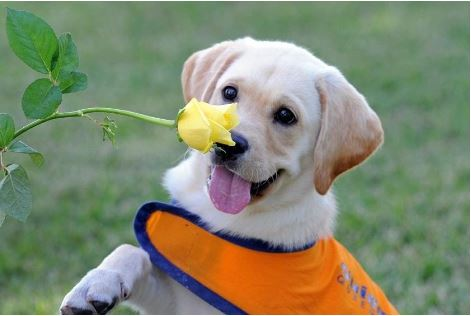
\includegraphics[width=0.45\textwidth,height=0.3\textwidth]{pictures/slic1.jpg} }}%
    \qquad
    \subfloat[Calculated Superpixel Boundaries]{{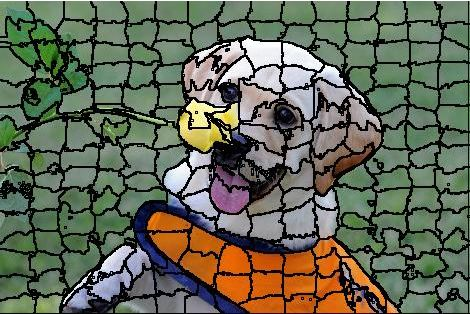
\includegraphics[width=0.45\textwidth,height=0.3\textwidth]{pictures/slic2.jpg} }}%
    
    \subfloat[Recolored image]{{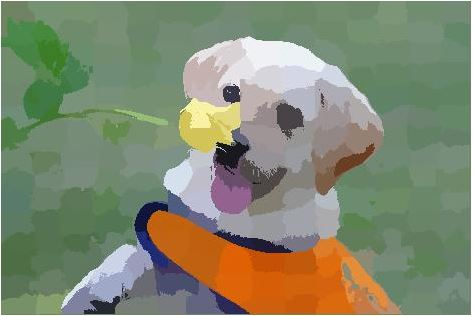
\includegraphics[width=0.45\textwidth,height=0.3\textwidth]{pictures/slic3.jpg} }}%
    
    \caption{Original image and segmented image}%
    \label{superpixel}%
\end{figure}
\noindent
In the segmented image, each region is identified by a boundary as shown. Here each region is shown with a single color rather than the color of all pixels. This single color can be found by calculating mean of the all pixels of that region. This color is used as a substitute of all colors of that region.


\section{Finding Global Contrast Map}
 We use the most widely used prior, i.e., the contrast prior ,which means that the color components belonging to a salient object often have strong contrast to their surroundings. Similarity  between two regions r\textsubscript{i},r\textsubscript{j},\textit{i,j=1.2.....N} is calculated by equation \eqref{1}. where ci and cj are the average color vector of the regions in LAB color space, σ is a constant which controls the strength of the weight and d is a distance function which calculates color based similarity between regions.
 
 \begin{equation}\label{1}
d\textsubscript{c}(r\textsubscript{i},r\textsubscript{j})&= e^{-\frac{||c\tectsubscript{i}-c\textsubscript{j}||^2}{\sigma^2}}
\end{equation}
\noindent
 But color dissimilarity is our main concern. So for this purpose we use equation \eqref{2}.
 
 \begin{equation}\label{2}
\rho \textsubscript{c}(r\textsubscript{i},r\textsubscript{j}) &= 1- d\textsubscript{c}(r\textsubscript{i},r\textsubscript{j}) 
\end{equation}
\noindent
 For every region r\textsubscript{i} This value from equation \eqref{2} is then averaged with every other superpixels of the image to get color priori based rarity of region r\textsubscript{i} Using equation \eqref{3}. 
 
 \begin{equation}\label{3}
s\textsubscript{c}(r\textsubscript{i}) &= \frac{1}{N} \sum_{k=1}^{N} \rho \textsubscript{c}(r\textsubscript{i},r\textsubscript{k})
\end{equation}

\begin{figure}[here]%
    \centering
    \subfloat[Original image]{{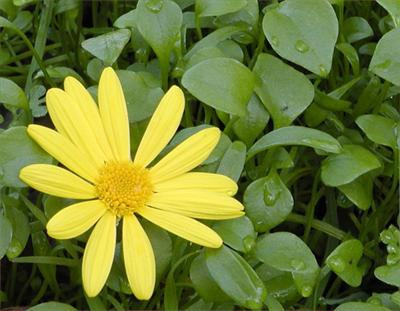
\includegraphics[width=0.45\textwidth,height=0.3\textwidth]{pictures/10841/color_image.jpg} }}%
    \qquad
    \subfloat[Global Contrast Map]{{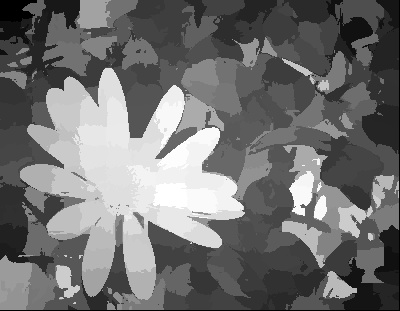
\includegraphics[width=0.45\textwidth,height=0.3\textwidth]{pictures/10841/globalsaliencyMap.jpg} }}%
    \caption{generated global contrast map}%
    \label{superpixel}%
\end{figure}
 \noindent
 image region with similar colors are likely to have the same label . However, this can produce false alarms when part of the background has a similar color to the foreground object. Therefore, we incorporate the spatial distance d\textsubscript{s} between regions normalized by the image size to down-weight the importance of distant regions according to the assumptions in Table 1\cite{masudsir2016}.
 We calculate d\textsubscript{s} by using equation \eqref{4} Where p\textsubscript{i} and p\textsubscript{j} are the average position vector of the regions r\textsubscript{i} and r\textsubscript{j} respectively. Equation \ref{5} defines the dissimilarity between two region r\textsubscript{i},r\textsubscript{j} including both color and spatial prior, where $\gamma$ is a constant used to avoid the division by zero and defined by equation \eqref{6}
 
\begin{equation}\label{4}
d\textsubscript{s}(r\textsubscript{i},r\textsubscript{j})&= ||p\textsubscript{i}-p\textsubscript{j}||^2
\end{equation}

\begin{equation}\label{5}
\rho \textsubscript{c,s}(r\textsubscript{i},r\textsubscript{j})&=  \frac{\rho\textsubscript{c}(r\textsubscript{i},r\textsubscript{j})}{d\textsubscript{s}(r\textsubscript{i},r\textsubscript{j})+\gamma}
\end{equation}
 
 
\begin{equation}\label{6}
\gamma &= 1-e^\frac{1}{\sigma^2}
\end{equation}
\noindent
and finally equation \eqref{6} gives the global saliency value of a region r\textsubscript{i} after comparing it with all other regions of the image. Fig. 3.2(b) shows the global contrast map\cite{masudsir2016} of the Fig. 1(a) generated by equation \ref{6}.









\begin{equation}\label{7}
S\textsubscript{G}(r\textsubscript{i}) &= \frac{1}{N} \sum_{k=1}^{N} \rho \textsubscript{c,s}(r\textsubscript{i},r\textsubscript{k})
\end{equation}





 
{\rowcolors{3}{green!80!yellow!50}{green!70!yellow!40}

\begin{tabular}{ |p{3cm}|p{3cm}|p{3cm}|  }
\hline
\multicolumn{3}{|c|}{Table 1: Saliency proportionality for color and distance} \\
\hline
Color Distance & Spatial Distance & Saliency \\
\hline
Low & Near & Low  \\
Low & Far   & Low  \\
High & Near & High  \\
High & Far & X \\
\hline
\end{tabular}
}

\section{Boundary Aware Contrast Map}
Global contrast map works nicely if  the background is more simple smooth . but when the background will be complex global contrast priori can not eliminate background fully .To solve this  problem boundary awareness\cite{masudsir2016} is needed where each region is compared with other regions that touches the boundary to find the difference of color. Let's consider there are M number of regions that touches the border. We take every region r\textsubscript{i}  and compare it's color difference with those M regions and store the value in a vector. equation \eqref{8} is used to do this job.here r\textsubscript{i} denotes each region b\textsubscript{j} denotes the regions that touches border. $\rho$\textsubscript{c,s} denotes the color and spatial dissimilarity between each region and boundary regions. 

\begin{equation}\label{8}
B\textsubscript{i}[j] &= \rho\textsubscript{c,s}(r\textsubscript{i},b\textsubscript{j})
\end{equation}


\noindent
Data after the calculation is stored in B\textsubscript{i} which is the color dissimilarity vector.this vector is then sorted in ascending order using equatio \eqref{9}.

\begin{equation}\label{9}
B\textsubscript{i} &= sort(B\textsubscript{i})
\end{equation}
\noindent
we sort the vector so that the small values (that represents less difference in color) stays in front of the vector and thereby it becomes easier to select the desired
range of values. Finally, the boundary aware saliency value of r\textsubscript{i} is assigned by using equation \eqref{10}, where 0 <$\alpha$< 1. By equation \eqref{10}, we are actually taking the average of $\alpha$M minimal dissimilarity (i.e., to some extent similar) values with the assumption that a region similar to the boundary regions will generally produce a very lower measure and thereby suppress the background regions.


\begin{figure}%
    \centering
    \subfloat[Global Contrast Map]{{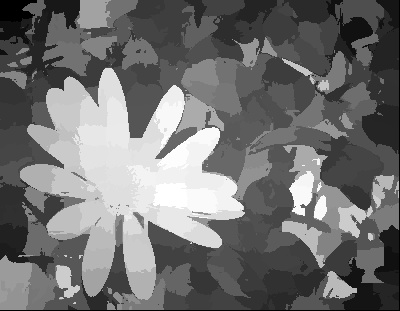
\includegraphics[width=0.45\textwidth,height=0.3\textwidth]{pictures/10841/globalsaliencyMap.jpg} }}%
    \qquad
    \subfloat[Bondary Aware Contrast Map]{{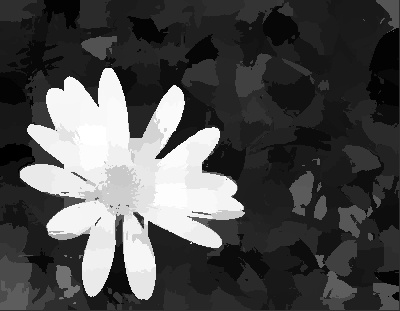
\includegraphics[width=0.45\textwidth,height=0.3\textwidth]{pictures/10841/BoundarysaliencyMap.jpg} }}%
    \caption{generated boundary aware contrast map}%
    \label{superpixel}%
\end{figure}
 


\begin{equation}\label{10}
S\textsubscript{B}(r\textsubscript{i}) &=\frac{1}{\alpha M} \sum_{k=1}^{\alpha M} B\textsubscript{i}k
\end{equation}

\noindent
For example if we consider 4 regions that touches the border and we want to calculate the value of region r\textsubscript{i} then using equation \eqref{8} we will get four values. Say those values are 0.45,0.37,0.52,0.63. after applying equation \eqref{9} the color dissimilarity vector will have 0.37,0.45,0.52,0.63 in ascending order. Now if we consider $\alpha$ = 0.5 then first two item will be chosen and and the average of those will be 0.41 and if we consider another region which after following the same procedure gives 0.21 as output then we can assume that the first region with value 0.41 is more salient than the region with value 0.21







\section{Color Saliency}

Color saliency of an image is defined by distinctness of color in an image. The more the region have more distinct color it is considered as more salient that means more the probability of being foreground and the region which have less distinct color it is considered as less salient and as a result more probability of being background. In this thesis we proposed a simple method for finding color saliency of an image. To get the distinct color we take the difference of mean color from the image as a result a region having low color frequency can be found.

\subsection{Lab Color Space}
The Lab color space describes mathematically all perceivable colors in the three dimensions L for lightness and a and b for the color components green–red and blue–yellow. The terminology "Lab" originates from the Hunter 1948 color space.[1][2] Nowadays "Lab" is frequently mis-used as abbreviation for CIEL*a*b* 1976 color space (also CIELAB); the asterisks/stars distinguish the CIE version from Hunter's original version. The difference from the Hunter Lab coordinates is that the CIELAB coordinates are created by a cube root transformation of the CIE XYZ color data, while the Hunter Lab coordinates are the result of a square root transformation. Other, less common examples of color spaces with Lab representations make use of the CIE 1994 color difference and the CIE 2000 color difference.The Lab color space exceeds the gamuts of the RGB and CMYK color models (for example, ProPhoto RGB includes about 90 percent all perceivable colors). One of the most important attributes of the Lab model is device independence. This means that the colors are defined independent of their nature of creation or the device they are displayed on. The Lab color space is used when graphics for print have to be converted from RGB to CMYK, as the Lab gamut includes both the RGB and CMYK gamut. Also it is used as an interchange format between different devices as for its device independence. The space itself is a three-dimensional real number space, that contains an infinite number of possible representations of colors. However, in practice, the space is usually mapped onto a three-dimensional integer space for device-independent digital representation, and for these reasons, the L*, a*, and b* values are usually absolute, with a pre-defined range. The lightness, L*, represents the darkest black at L* = 0, and the brightest white at L* = 100. The color channels, a* and b*, will represent true neutral gray values at a* = 0 and b* = 0. The red/green opponent colors are represented along the a* axis, with green at negative a* values and red at positive a* values. The yellow/blue opponent colors are represented along the b* axis, with blue at negative b* values and yellow at positive b* values. The scaling and limits of the a* and b* axes will depend on the specific implementation of Lab color, as described below, but they often run in the range of ±100 or −128 to +127 (signed 8-bit integer).

\subsection{Average Color Lab Image}
At first an image is converted into lab color image.Figure ~\ref{fig:conversion} shows the conversion from input to output image.Lab image has three channel and they are L-channel, a-channel, b-channel.Now mean, mode and average color is calculated separately for l-channel, a-channel and b-channel.Then global average color 
 C\textsubscript{avg} &= [L\textsubscript{avg},a\textsubscript{avg},b\textsubscript{avg}] in 
each channel is calculated from equation \ref{10}, \ref{11}, \ref{12}. 

\begin{equation}\label{10}
L\textsubscript{avg} &=min(\frac{(L\textsubscript{mean}+L\textsubscript{mode})}{2},L\textsubscript{mean})
\end{equation}

\begin{equation}\label{11}
a\textsubscript{avg} &=\frac{(a\textsubscript{mean}+a\textsubscript{mode})}{2}
\end{equation}

\begin{equation}\label{12}
b\textsubscript{avg} &=\frac{(b\textsubscript{mean}+b\textsubscript{mode})}{2}
\end{equation}


\begin{figure}[here]%
    \centering
    \subfloat[Input image]{{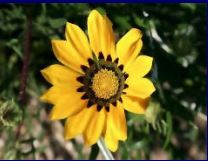
\includegraphics[width=0.45\textwidth,height=0.3\textwidth]{pictures/color_sal/1.jpg} }}%
    \qquad
    \subfloat[Lab image]{{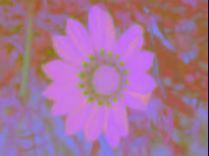
\includegraphics[width=0.45\textwidth,height=0.3\textwidth]{pictures/color_sal/2.jpg} }}%
    \caption{Conversion from input to lab image}%
    \label{fig:conversion}%
\end{figure}

\begin{figure}[here]%
    \centering
    \subfloat[l-channel]{{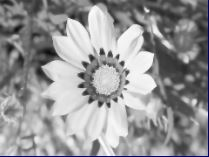
\includegraphics[width=0.45\textwidth,height=0.3\textwidth]{pictures/color_sal/3.jpg} }}%
    \qquad
    \subfloat[a-channel]{{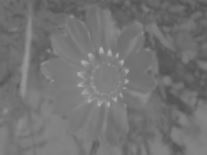
\includegraphics[width=0.45\textwidth,height=0.3\textwidth]{pictures/color_sal/4.jpg} }}%
    \qquad
    \subfloat[b-channel]{{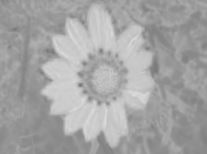
\includegraphics[width=0.45\textwidth,height=0.3\textwidth]{pictures/color_sal/5.jpg} }}%
    \caption{Different channel image in lab image}%
    \label{fig:conversion}%
\end{figure}

\subsection{Absolute Difference Lab Image}
Average color vector now used to compute absolute difference lab image.For each pixel having row x and column y 
absolute difference between that pixels intensity in three channel and average intensity in L-channel,a-channel and b-channel is calculated using equation \ref{13}

for L-channel
\begin{equation}\label{13}
DI\textsubscript{L}(x,y) &= |(I\textsubscript{L}(x,y) - L\textsubscript{avg})|
\end{equation}


for a-channel
\begin{equation}\label{14}
DI\textsubscript{a}(x,y) &= |(I\textsubscript{a}(x,y) - a\textsubscript{avg})|
\end{equation}


for b-channel
\begin{equation}\label{15}
DI\textsubscript{b}(x,y) &= |(I\textsubscript{b}(x,y) - b\textsubscript{avg})|
\end{equation}

Combing these three equation it can be written as vector equation \ref{16}


\begin{equation}\label{16}
DI\textsubscript{Lab}(x,y) &= |(I\textsubscript{Lab}(x,y) - C\textsubscript{avg})|
\end{equation}


\begin{figure}[here]%
    \centering
    \subfloat[Diff. Lab Image]{{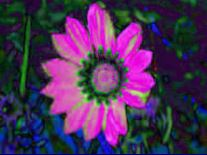
\includegraphics[width=0.45\textwidth,height=0.3\textwidth]{pictures/color_sal/6diff.jpg} }}%
    \qquad
    \subfloat[Diff. L-channel]{{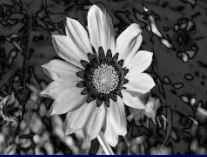
\includegraphics[width=0.45\textwidth,height=0.3\textwidth]{pictures/color_sal/diff3.jpg} }}%
    \qquad
    \subfloat[Diff. a-channel]{{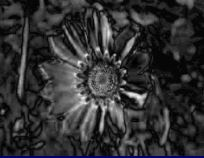
\includegraphics[width=0.45\textwidth,height=0.3\textwidth]{pictures/color_sal/diff4.jpg} }}%
    \qquad
    \subfloat[Diff. b-channel]{{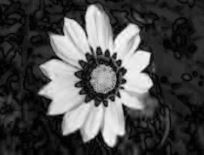
\includegraphics[width=0.45\textwidth,height=0.3\textwidth]{pictures/color_sal/diff5.jpg} }}%
    \caption{Absolute Difference lab image}%
    \label{fig:conversion}%
\end{figure}


\subsection{Color Map}
Final color map is the combination of three image. These three images are absolute difference L-channel, a-channel, b-channel images.
These three image are combined by weighted combination of their intensity values to get two images of single channel. Three channel image thus converted into single channel image using following equation  to get M,N 


\begin{equation}\label{17}
M\textsubscript{gray}(x,y) &= w\textsubscript{L}DI\textsubscript{L}(x,y) +w\textsubscript{a}DI\textsubscript{a}(x,y)+w\textsubscript{b}DI\textsubscript{b}(x,y) 
\end{equation}


\begin{equation}\label{18}
N\textsubscript{gray}(x,y) &= \sqrt{DI\textsubscript{L}^2(x,y)+DI\textsubscript{a}^2(x,y)+DI\textsubscript{b}^2(x,y)}
\end{equation}

here M is an image of single channel. Three channel L-channel,a-channel,b-channel are combined by weight w\textsubscript{L}, 
w\textsubscript{a} and w\textsubscript{b}. N is an single channel image combined by taking squared sum of three channel intensity values.
Final color Map is extracted by combining M and N image by equation \ref{20}

\begin{equation}\label{20}
MAP\textsubscript{color}(x,y) &= M^\gamma * N(x,y) 
\end{equation}
All the images are normalized after pixel level calculation. After getting median filter on MAP image it's saliency is calculated.


\subsection{Color Saliency Calculation}
Color saliency defines the most salient color of the image. If saliency is high then that pixel or region is most 
salient or foreground and if slaiency is low then that pixel or region is background or non-salient object. To find out the color saliency at first color map image is segmented by same number of region as original image. Then each region average value is calculated. Average intensity value is calculated by dividing sum of all pixels intensity in a region with the number of pexels in the region. Later saliency is calculated by dividing the average value by 255. Normalizing the value saliency will range from 0 to 1 for a region. Saliency value 1 means that region is most salient and its value 0 means that region is non salient.

\begin{figure}[t]%
    \centering
    \subfloat[N image]{{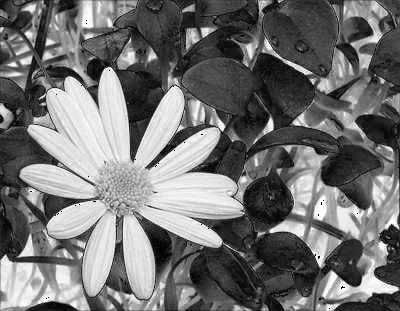
\includegraphics[width=0.3\textwidth,height=0.2\textwidth]{pictures/10841/N_xy.jpg} }}%
    \qquad
    \subfloat[M image]{{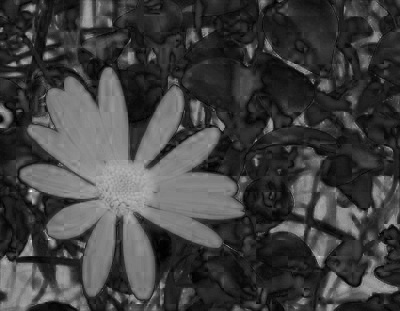
\includegraphics[width=0.3\textwidth,height=0.2\textwidth]{pictures/10841/g_xy.jpg} }}%
    \qquad
    \subfloat[Color Map]{{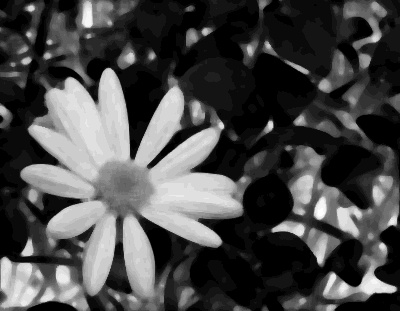
\includegraphics[width=0.3\textwidth,height=0.2\textwidth]{pictures/10841/median.jpg} }}%
    \qquad
    \subfloat[Color Saliency]{{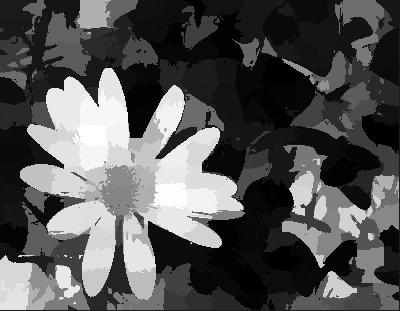
\includegraphics[width=0.3\textwidth,height=0.2\textwidth]{pictures/10841/COLORSALIENCY.jpg} }}%
    \caption{Construction of Color Saliency}%
    \label{fig:conversion23}%
\end{figure}


\section{Final Saliency Map}
Based on the three above mentioned saliency measurements we define the final saliency of a region r\textsubscript{i}, where Sal(ri) is normalized to the range [0,1] afterwards. For combining each map is given different level of  priority to gain better result. Equation \eqref{21} is used to compute the final saliency.



\begin{equation}\label{21}
Sal(r\textsubscript{i}) &=S\textsubscript{B}(r\textsubscript{i})\times W\textsubscript{B}+ S\textsubscript{G}(r\textsubscript{i}) \times W\textsubscript{G}+ S\textsubscript{C}(r\textsubscript{i}) \times W\textsubscript{C}
\end{equation}




\begin{figure}[here]%
    \centering
    \subfloat[Final Saliency Map 
    without smoothing]{{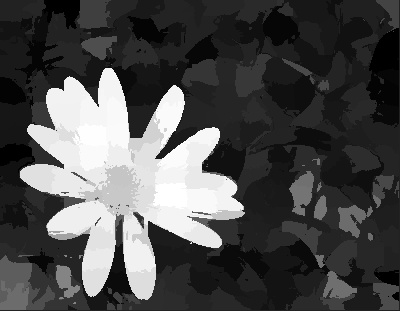
\includegraphics[width=0.45\textwidth,height=0.3\textwidth]{pictures/10841/FinalsaliencyMapWithoutSmoothing.jpg} }}%
    \qquad
    \subfloat[Final Saliency Map 
    with smoothing]{{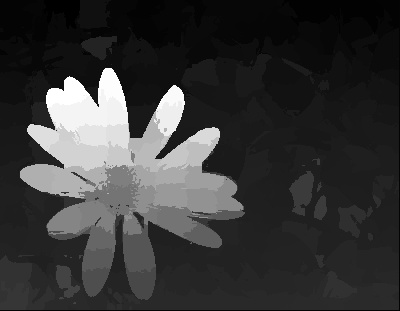
\includegraphics[width=0.45\textwidth,height=0.3\textwidth]{pictures/10841/FinalsaliencyMapWithSmoothing.jpg} }}%
    \caption{Generated final saliency map}%
    \label{superpixel}%
\end{figure}
\noindent
Here W\textsubscript{B}, W\textsubscript{G} and W\textsubscript{C} are different weights to adjust different saliency maps importance.
the output of equation \eqref{21} is then normalized to the range [0,1]

Our final workflow is shown in figure:3.9 
As we can see in the flowchart first an image is taken as input then it is divided into segments. Before dividing it from input image a color importance map is also calculated.
\begin{figure}[here]
  \centering
  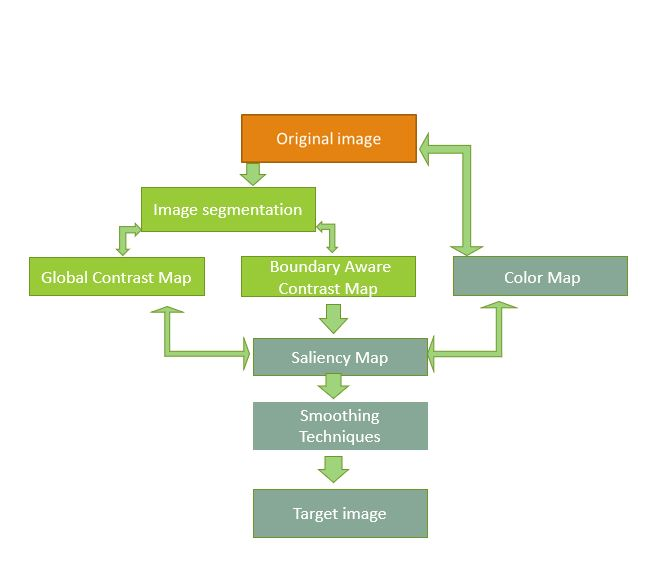
\includegraphics[width=0.7\textwidth,height=0.9\textwidth]{pictures/flowchart.jpg}
  \caption{Flow Diagram of The Process}
  \label{orangeleaf}
\end{figure}

\noindent
Now from the segmented image Global contrast map is calculated and Boundary aware contrast map is also calculated. Then combining these two maps along with the previously built color importance map gives us the saliecy map. We then apply some smoothing technique to make our result better. Then after applying smoothing technique our final output image is generated.

